% This file was created by matlab2tikz.
%
%The latest updates can be retrieved from
%  http://www.mathworks.com/matlabcentral/fileexchange/22022-matlab2tikz-matlab2tikz
%where you can also make suggestions and rate matlab2tikz.
%
\definecolor{mycolor1}{rgb}{0.49412,0.18431,0.55686}%
\definecolor{mycolor2}{rgb}{1.00000,0.41176,0.16078}%
%
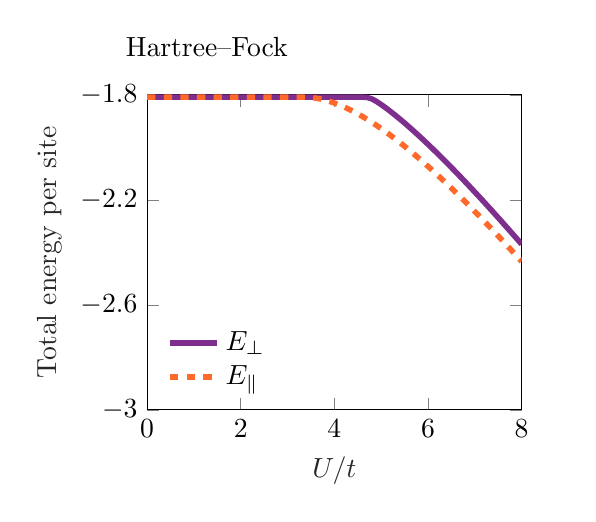
\begin{tikzpicture}

\begin{axis}[%
width=4.755cm,
height=4cm,
at={(0cm,0cm)},
scale only axis,
xmin=0,
xmax=8,
xlabel style={font=\color{white!15!black}},
xlabel={$U/t$},
ymin=-3,
ymax=-1.8,
ytick={-3,-2.6,-2.2,-1.8},
ylabel style={font=\color{white!15!black}},
ylabel={Total energy per site},
axis background/.style={fill=white},
legend style={at={(0.03,0.03)}, anchor=south west, legend cell align=left, align=left, fill=none, draw=none}
]
\addplot [color=mycolor1, line width=2.0pt]
  table[row sep=crcr]{%
0	-1.80871598398\\
0.1	-1.80871598398\\
0.2	-1.80871598398\\
0.3	-1.808715983979\\
0.4	-1.808715983979\\
0.5	-1.808715983979\\
0.6	-1.808715983979\\
0.7	-1.808715983979\\
0.8	-1.808715983979\\
0.9	-1.808715983978\\
1	-1.808715983978\\
1.1	-1.808715983977\\
1.2	-1.808715983978\\
1.3	-1.808715983975\\
1.4	-1.808715983975\\
1.5	-1.808715983976\\
1.6	-1.808715983972\\
1.7	-1.808715983973\\
1.8	-1.808715983973\\
1.9	-1.808715983973\\
2	-1.808715983973\\
2.1	-1.808715983972\\
2.2	-1.808715983971\\
2.3	-1.808715983969\\
2.4	-1.808715983966\\
2.5	-1.808715983962\\
2.6	-1.808715983957\\
2.7	-1.80871598396\\
2.8	-1.808715983961\\
2.9	-1.808715983951\\
3	-1.808715983948\\
3.1	-1.808715983943\\
3.2	-1.808715983946\\
3.3	-1.808715983945\\
3.4	-1.808715983939\\
3.5	-1.808715983939\\
3.6	-1.80871598393\\
3.7	-1.808715983924\\
3.8	-1.808715983915\\
3.9	-1.808715983913\\
4	-1.808715983908\\
4.1	-1.808715983908\\
4.2	-1.808715983896\\
4.3	-1.808715983893\\
4.4	-1.808715983885\\
4.5	-1.808715983875\\
4.6	-1.808715983873\\
4.7	-1.809842785042\\
4.8	-1.815298006678\\
4.9	-1.825064035483\\
5	-1.836948945101\\
5.1	-1.849785797503\\
5.2	-1.863335294966\\
5.3	-1.877471313266\\
5.4	-1.892120145318\\
5.5	-1.907226674128\\
5.6	-1.922744422195\\
5.7	-1.938638253552\\
5.8	-1.954878735192\\
5.9	-1.971444695877\\
6	-1.98830705282\\
6.1	-2.005454023541\\
6.2	-2.0228611756\\
6.3	-2.040520959567\\
6.4	-2.058415504732\\
6.5	-2.076528746018\\
6.6	-2.09485685702\\
6.7	-2.113385267507\\
6.8	-2.132100306467\\
6.9	-2.151001378088\\
7	-2.170075720028\\
7.1	-2.189315573458\\
7.2	-2.208709343686\\
7.3	-2.228259326102\\
7.4	-2.247954413231\\
7.5	-2.267788631129\\
7.6	-2.287756364297\\
7.7	-2.307847520568\\
7.8	-2.328067034941\\
7.9	-2.348405029644\\
8	-2.368857029091\\
};
\addlegendentry{$E_\perp$}

\addplot [color=mycolor2, dashed, line width=2.0pt]
  table[row sep=crcr]{%
0	-1.80871598398\\
0.1	-1.80871598398\\
0.2	-1.80871598398\\
0.3	-1.80871598398\\
0.4	-1.808715983979\\
0.5	-1.808715983978\\
0.6	-1.808715983979\\
0.7	-1.808715983978\\
0.8	-1.808715983975\\
0.9	-1.808715983975\\
1	-1.808715983974\\
1.1	-1.808715983974\\
1.2	-1.808715983972\\
1.3	-1.80871598397\\
1.4	-1.808715983967\\
1.5	-1.808715983961\\
1.6	-1.808715983965\\
1.7	-1.808715983956\\
1.8	-1.808715983957\\
1.9	-1.808715983955\\
2	-1.808715983949\\
2.1	-1.808715983938\\
2.2	-1.808715983936\\
2.3	-1.808715983925\\
2.4	-1.808715983921\\
2.5	-1.808715983919\\
2.6	-1.808715983915\\
2.7	-1.808715983901\\
2.8	-1.808715983896\\
2.9	-1.808715983879\\
3	-1.808715983867\\
3.1	-1.808715983848\\
3.2	-1.808715983836\\
3.3	-1.808715983824\\
3.4	-1.808861311998\\
3.5	-1.810032932008\\
3.6	-1.812309813344\\
3.7	-1.815619085283\\
3.8	-1.819895304948\\
3.9	-1.825077265936\\
4	-1.831107881559\\
4.1	-1.83793498179\\
4.2	-1.845513515807\\
4.3	-1.853796207794\\
4.4	-1.862744752609\\
4.5	-1.872319221759\\
4.6	-1.882487532685\\
4.7	-1.893214484291\\
4.8	-1.9044667749\\
4.9	-1.916222419854\\
5	-1.928455706775\\
5.1	-1.941135346322\\
5.2	-1.954241744559\\
5.3	-1.967757330694\\
5.4	-1.981654998818\\
5.5	-1.995919217375\\
5.6	-2.010537151826\\
5.7	-2.02548782571\\
5.8	-2.040752132505\\
5.9	-2.056323499055\\
6	-2.072184061086\\
6.1	-2.088317195308\\
6.2	-2.104718800377\\
6.3	-2.121373211923\\
6.4	-2.138269654514\\
6.5	-2.155394198694\\
6.6	-2.172745067087\\
6.7	-2.190309015555\\
6.8	-2.208077417525\\
6.9	-2.226042102134\\
7	-2.24419158919\\
7.1	-2.2625262802\\
7.2	-2.28103514755\\
7.3	-2.299711558258\\
7.4	-2.318549210711\\
7.5	-2.337542110775\\
7.6	-2.356684553544\\
7.7	-2.375971106356\\
7.8	-2.395393229444\\
7.9	-2.414952921328\\
8	-2.43464189184\\
};
\addlegendentry{$E_\parallel$}

\end{axis}

\begin{axis}[%
width=6.135cm,
height=4.908cm,
at={(-0.798cm,-0.54cm)},
scale only axis,
xmin=0,
xmax=1,
ymin=0,
ymax=1,
axis line style={draw=none},
ticks=none,
axis x line*=bottom,
axis y line*=left
]
\end{axis}

\node[above left]
at (current bounding box.north) {Hartree--Fock};

\end{tikzpicture}%
